% !TEX spellcheck = en_US
% !TeX root = Lecture.tex
%---------------------------------------------------------------------------------
\section[Wind Energy Extraction]{Optimal Wind Energy Extraction}\label{sec:WEN}
%---------------------------------------------------------------------------------
\miniframesoff	
\begin{frame}<handout:0>[noframenumbering]{Content}
\tableofcontents[currentsection]
\PutAt<1-|handout:0>[5cm]{(10cm,2cm)}{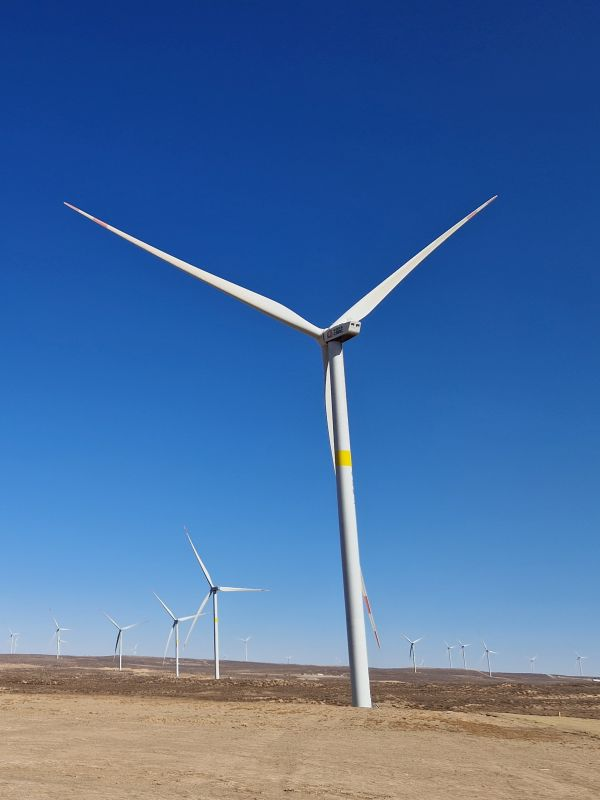
\includegraphics[width=4.0cm]{\StylePath/content/Gobi}} % graphic related to topic	
\end{frame}
\miniframeson
%---------------------------------------------------------------------------------
%---------------------------------------------------------------------------------
\begin{frame}{Wind Energy and Power} 
\setlength{\abovedisplayskip}{0pt}
\setlength{\belowdisplayskip}{0pt}
\begin{columns}
	\column{9cm} 
	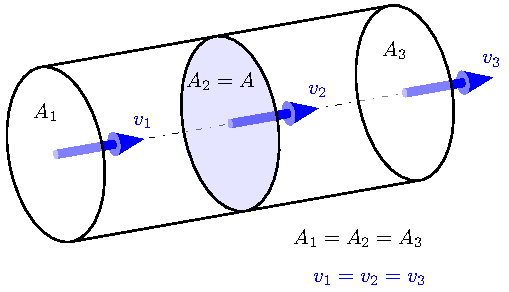
\includegraphics[width=\linewidth]{WEN/streamtube1.pdf}		
	\column{5cm}
	\begin{block}<1->{Kinetic Energy}
		\begin{align*}
		E   & = \frac{1}{2} m v_1^2
		\end{align*}
		\begin{tabular}{ll}
			$m$ 	&  air mass\\
			$v_1$ 	&  undisturbed wind speed
		\end{tabular}
	\end{block}	
	%---
	\begin{block}<2->{Mass Flow}
		\begin{align*}
		\dot m & = \rho A v_1
		\end{align*}
		\begin{tabular}{ll}
			$\rho $ 	&  air density\\
			$A$ 		&  control area
		\end{tabular}	
	\end{block}	
	%---
	\begin{block}<3->{Wind Power}
		\begin{align*}
		P_{\textnormal{Wind}}=\dot E = \frac{1}{2} \rho A v_1^3 
		\end{align*}
	\end{block}	
	%---	
\end{columns} 	
\end{frame}
%---------------------------------------------------------------------------------
\begin{frame}{Energy Extraction by Deceleration} 
\begin{figure}[htbp]
	\begin{center}
		\begin{minipage}[c]{0.4\linewidth}
			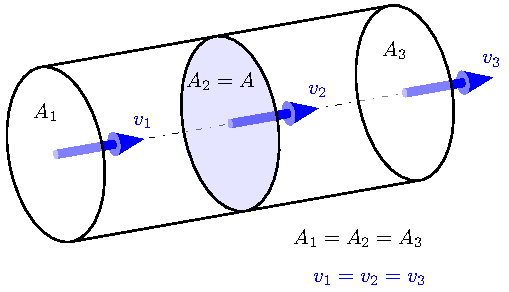
\includegraphics[width=\linewidth]{WEN/streamtube1.pdf}
		\end{minipage}
		\visible<2->{
		\begin{minipage}[c]{0.4\linewidth}
			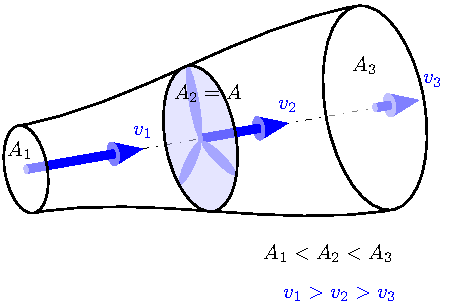
\includegraphics[width=\linewidth]{WEN/streamtube2.pdf}
		\end{minipage}
		}
		\begin{minipage}[c]{0.15\linewidth}
			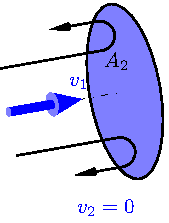
\includegraphics[width=\linewidth]{WEN/streamtube3.pdf}
		\end{minipage}
	\end{center}
\end{figure}
\begin{block}<1->{}
\begin{itemize}
	\item energy can be extracted by decelerating the wind (wind energy converter)
	\item heavily idealized wind turbine without any losses analyzed by Betz
	\item no extraction with no or total deceleration
	\item <2-> Optimum must be somewhere in between!
	\item <2-> stream tube with divergent streamlines due to continuity: $\rho A_1 v_1= \rho A_2 v_2= \rho A_3 v_3$
\end{itemize}
\end{block}	 
\end{frame}
%---------------------------------------------------------------------------------
\begin{frame}{Pioneers of Wind-Power Technology} 
\begin{columns}
	\column{7cm}
	\centering
	\includegraphics<1->[height=4.9cm,trim=0 9.25cm 0 0, clip] {WEN/Hau2006Fig2.17}
	\begin{columns}
		\column{3.0cm} 
		\begin{block}<2->{}{Hydrogen from wind power}\end{block}	
		\column{3.0cm} 
		\begin{block}<2->{}{``Betz's law'', blade design}\end{block}	
	\end{columns}	
	\column{7cm}
	\centering	
	\includegraphics<3->[height=4.9cm,trim=0 0 0 9.25cm, clip] {WEN/Hau2006Fig2.17}
	\begin{columns}
		\column{3.0cm} 
		\begin{block}<4->{}{First MW wind turbine}\end{block}	
		\column{3.0cm} 
		\begin{block}<4->{}{First composite blades}\end{block}		
	\end{columns}		
\end{columns} 
\flushright\tiny\textcolor{gray}{\cite{Hau2006}}	
\end{frame}		 		 
%---------------------------------------------------------------------------------
\begin{frame}{Power Coefficient According to Betz} 
\setlength{\abovedisplayskip}{0pt}
\setlength{\belowdisplayskip}{1pt}
\begin{columns}
\column{8cm}
	%---	
	\begin{block}<1->{Extracted energy}
		\begin{align*}
		E   & = \frac{1}{2} m v_1^2 - \frac{1}{2} m v_3^2 = \frac{1}{2} m (v_1^2 - v_3^2)
		\end{align*}
	\end{block}	
	%---	
	\vspace*{-1pt}
	%---
	\begin{block}<2->{Extracted power}
		\begin{align*}
		P   & = \frac{1}{2} \dot m (v_1^2 - v_3^2) \quad\textnormal{with}\quad v_2=\frac{v_1+v_3}{2}\\
		& = \underbrace{\frac{1}{2}\rho Av_1^3}_{P_{\textnormal{Wind}}}
		\underbrace{\frac{1}{2}\left(1+\frac{v_3}{v_1}\right)\left(1-\left(\frac{v_3}{v_1}\right)^2\right)}_{c_{\textnormal{P}}}
		\end{align*}
	\end{block}	
	%---	
	\vspace*{-1pt}
	%---	
	\begin{block}<3->{Power coefficient $c_{\textnormal{P}}$ and axial induction $a$}
		\begin{align*}
		c_{\textnormal{P}} = \frac{P}{P_{\textnormal{Wind}}} = 4a(1-a)^2 \quad\textnormal{with}\quad 1-a=\frac{v_2}{v_1}
		\end{align*}
	\end{block}	
	%---
	%---	
\column{6cm} 
	\centering
	\includegraphics<3->[width=6cm] {WEN/BetzOptimum.pdf}
	\begin{block}<3->{}
		Maximum $c_{\textnormal{P}}=\frac{16}{27}$ at $\frac{v_3}{v_1}=\frac{1}{3}$ and $a=\frac{1}{3}$
	\end{block}			
\end{columns} 
\end{frame}
%---------------------------------------------------------------------------------
\begin{frame}{Power Coefficient According to Betz} 
\setlength{\abovedisplayskip}{0pt}
\setlength{\belowdisplayskip}{1pt}
	\begin{block}<1->{Power Coefficient $c_{\textnormal{P}}$}
		\begin{align*}
		c_{\textnormal{P}} & = \frac{P}{P_{\textnormal{Wind}}} = \frac{1}{2} \left( 1 + \frac{v_3}{v_1} \right) \left( 1 - \left( \frac{v_3}{v_1} \right)^2 \right) \text{\ with\ } x=\frac{v_3}{v_1}\\
		& = \frac{1}{2} (1+x)(1-x^2)=\frac{1}{2}(-x^3-x^2+x+1)
		\end{align*}
	\end{block}	
	%---	
	\vspace*{-1pt}
	%---
	\begin{block}<2->{Derivation of $c_{\textnormal{P}}$}
		\begin{align*}
		c_{\textnormal{P}}' &= \frac{\textnormal{d} c_{\textnormal{P}}}{\textnormal{d}x} = \frac{1}{2} \left( - 3 x^2 - 2 x +1 \right) = 0 \quad \Rightarrow \quad x=\frac{v_3}{v_1} = \frac{1}{3}
		\end{align*}
	\end{block}
	%---	
	\vspace*{-1pt}
	%---
	\begin{block}<3->{Maximum of $c_{\textnormal{P}}$}
		\begin{align*}
		c_{\textnormal{P}} \left( \frac{v_3}{v_1} = \frac{1}{3} \right) &= \frac{1}{2} \left( 1 + \frac{1}{3} \right) \left( 1 - \left( \frac{1}{3} \right)^2 \right) = \frac{16}{27} \approx 59\%
		\end{align*}
	\end{block}
\end{frame}
%---------------------------------------------------------------------------------
\begin{frame}[t]{Thrust Coefficient According to Betz}
\setlength{\abovedisplayskip}{0pt}
\setlength{\belowdisplayskip}{1pt} 
\begin{columns}
\column{8cm}
	%---	
	\begin{block}<1->{Thrust force $T$}
		\begin{align*}
		T   &= \dot m  (v_1 - v_3)  \quad\textnormal{with}\quad v_2=\frac{v_1+v_3}{2}\\
		&= \underbrace{\frac{1}{2}\rho v_1^2}_{\textnormal{dynamic pressure}} A 
		\underbrace{\left(1-\left(\frac{v_3}{v_1}\right)^2\right)}_{c_{\textnormal{T} } }
		\end{align*}
	\end{block}	
	%---	
	\begin{block}<2->{Thrust coefficient $c_{\textnormal{T}}$ and axial induction $a$}
		\begin{align*}
		c_{\textnormal{T}} = 4a(1-a) \quad\textnormal{with}\quad 1-a=\frac{v_2}{v_1}
		\end{align*}
	\end{block}	
	%---
	%---	
\column{6cm} 
	\centering
	\includegraphics<3->[width=6cm] {WEN/BetzThrust.pdf}
	\begin{block}<3->{}
		\begin{itemize}
			\item $c_{\textnormal{T}}=\frac{8}{9}$ at $a=\frac{1}{3}$
			\item 	$c_{\textnormal{T}}\approx1.1$ for a circular disk\\
			\item[$\rightarrow$] in the optimal case thrust is similar to a solid disk
		\end{itemize}	
	\end{block}			
\end{columns} 
\end{frame}
%---------------------------------------------------------------------------------
\begin{frame}{Froude-Rankine Theorem}
\setlength{\abovedisplayskip}{0pt}
\setlength{\belowdisplayskip}{1pt} 
\begin{columns}
	\column{6cm} 
	\centering
	\includegraphics<1->[width=6cm] {WEN/Gasch2012Fig5.5.pdf}\\	
	\flushright\tiny\textcolor{gray}{\cite{Gasch2012a}}	
	\column{8cm}
	\begin{block}<1->{Theorem}
		\begin{align*}
	 		v_2=\frac{v_1+v_3}{2}
		\end{align*}
	\end{block}		
	\begin{block}<1->{Steps of proof}
		\begin{itemize}
			\item Express thrust $T$ by using the principle of linear momentum: $T=\dot{m}(v_1-v_3)$
			\item Apply Bernoulli Equation for plane left and plane right of the rotor
			\item Apply $v_{-2}=v_{+2}$ (continuity) and $p_1=p_3$. This leads to $\frac{\rho}{2} \left( v_1^2-v_3^2 \right) = p_{-2}-p_{+2}$
			\item Express Thrust as difference of static pressure, $T=A(p_{-2}-p_{+2})$, and apply $\dot{m}=\rho A v_2$
		\end{itemize}
	\end{block}	
\end{columns} 	
\end{frame}
%---------------------------------------------------------------------------------
\begin{frame}{Basic Concepts of Wind Energy Converters} 
\begin{columns}
	\column{9cm} 
		\centering
		\includegraphics<1->[width=9cm] {WEN/Gasch2012Fig3.1.pdf}\\	
		\flushright\tiny\textcolor{gray}{\cite{Gasch2012a}}	
	\column{5cm}
	\begin{block}<1->{Modern wind turbines}
		\begin{itemize}
		\item usually lift driven, horizontal, upwind turbines
		\item usually 3 blades best compromise between loads, energy and cost
		\item best turbines reach $c_{\textnormal{P}}=\SI{52}{\percent}$
		\item tip speed ratio $\lambda=\frac{v_{\textnormal{tip}}}{v_1}$ usually around $7$
		\item drag driven usually used for anemometers, $c_{\textnormal{P}}=\SI{10}{\percent}$
		\end{itemize}
	\end{block}	
\end{columns} 	
\end{frame}
%---------------------------------------------------------------------------------